\chapter{Manual de Instalación}

\begin{center}
	\textbf{Preparado por:} Juan Omar Huanca Balboa
\end{center}

\section{Introducción}

La plataforma web educativa cuenta con un espacio que necesita ser instalado y configurado.

Los requerimientos mínimos necesarios para esto son.

\begin{itemize}

\item Ubuntu 16.04.
\item 2 GB de RAM.
\item 30 GB Disco Duro.

\end{itemize}

La plataforma se encuentra desarrollo en lenguaje servidor PHP y tiene como 
persistencia definida una base de datos en MySQL.

\section{Instalación}

Acerca de, la instalación de utilitarios (git), servidor web, servidor de bases de
datos.

Ahora se describe el proceso de instalación, por el mismo se pide disponer
de una conexión a Internet; de igual manera, la cuenta de super usuario 
\textquotedouble{root}.

\begin{itemize}

\item MySQLServer v14.14
\item Apache2 v2.4.18
\item PhpMyAdmin v
\item PHP v7.0
\item GIT v
\end{itemize}

\subsection{MySQL server} \label{ssec:mysqlServer}

Abrir una terminal y ejecutar las sentencias.

\begin{lstlisting}[language=bash, caption={Comando para instalación de gestor de base de datos}]
# apt-get update
# apt-get install mysql-server 
\end{lstlisting}

Así mismo, ingresar la contraseña del usuario privilegiado denominado 
\textquotedouble{super usuario}. Se utilizara la contraseña 
\textquotedouble{root}.

\begin{figure}[!ht]
\centering
	\fbox{
		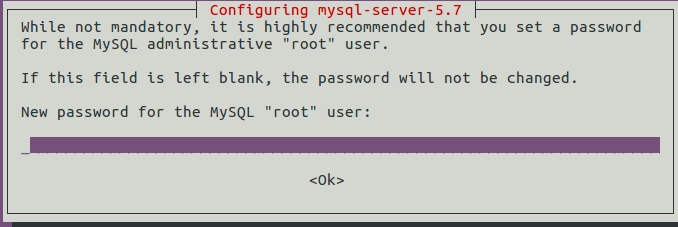
\includegraphics[scale=0.5]{passwordMySQLServer}
	}	\caption{Formulario de registro de contraseña para super usuario}
\end{figure}

\subsection{Apache2}

Acerca de, la instalacion de un servidor web para mostrar la aplicación web.

\begin{lstlisting}[language=bash, caption={Comando para instalación de servidor web}]
# apt-get install apache2 
\end{lstlisting}

como se afirmo arriba, se procede a realizar la verificación de la instalación
por uso de un navegador web, para luego escribir \textquotedouble{http://localhost}. 

\begin{figure}[!ht]
\centering
	\fbox{
		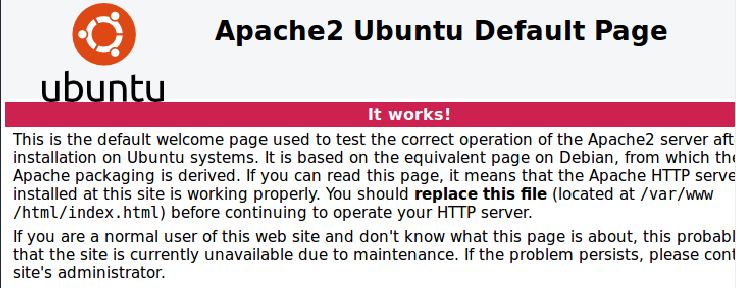
\includegraphics[scale=0.5]{verifyApacheBrowser}
	}	\caption{Verificación ejecución página por defecto de apache}
\end{figure}


\subsection{PhpMyAdmin}

En cuanto a, cliente para el servidor de base de datos, realizar la ejecución
del comando.

\begin{lstlisting}[language=bash, caption={Comando para instalación de cliente para base de datos}]
# apt-get install phpmyadmin 
\end{lstlisting}

Con respecto al primer punto, en el proceso de instalación pide la selección
de un servidor web, presionar la tecla \textquotedouble{Tab} y pinchar sobre
el botón \textquotedouble{Ok}.

\begin{figure}[!ht]
\centering
	\fbox{
		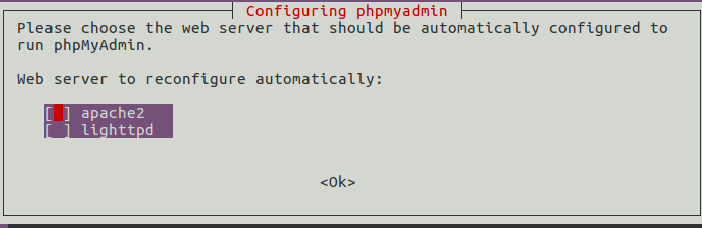
\includegraphics[scale=0.5]{chooseApachePhpMyAdmin}
	}	\caption{Formulario de selección de tipo de servidor web}
\end{figure}

Ahora bien, se tiene que escribir la misma contraseña definido en la sección
\ref{ssec:mysqlServer} y pinchar sobre el botón \textquotedouble{Ok}.

\begin{figure}[H]
\centering
	\fbox{
		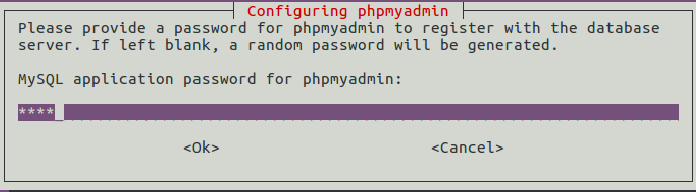
\includegraphics[scale=0.5]{formPasswordPhpMyAdmin}
	}	\caption{Formulario de ingreso de contraseña para cliente de base de datos}
\end{figure}

Mas aun, escribir nuevamente la contraseña definida en el paso anterior.

\begin{figure}[!ht]
\centering
	\fbox{
		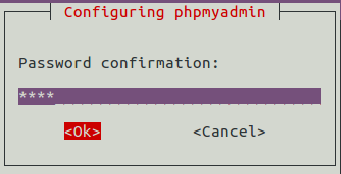
\includegraphics[scale=0.5]{formConfirmPasswordPhpMyAdmin}
	}	\caption{Formulario de confirmación de contraseña para cliente de base de datos}
\end{figure}

En relación con el funcionamiento de el cliente de base de datos, se sugiere
realizar la verificación de la instalación, por lo cual se tiene que abrir un
navegador web y escribir en la dirección URL 
\textquotedouble{http://localhost/phpmyadmin}.

\begin{figure}[!ht]
\centering
	\fbox{
		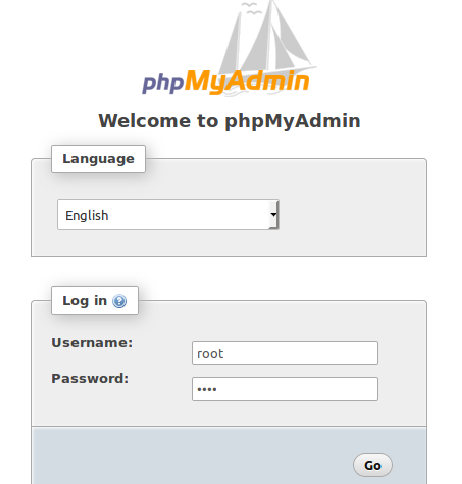
\includegraphics[scale=0.5]{verifyPhpMyAdminBrowser}
	}	\caption{Verificación ejecución página por defecto de apache}
\end{figure}

\subsection{PHP}

Por lo que se refiere a, lenguaje lado del servidor.

\begin{lstlisting}[language=bash, caption={Comando para instalación de lenguaje en el lado del servidor}]
# apt-get install php 
\end{lstlisting}

Con respecto al primer punto, en el proceso de instalación pide la selección
de un servidor web, presionar la tecla \textquotedouble{Tab} y pinchar sobre
el botón \textquotedouble{Ok}.

\begin{figure}[!ht]
\centering
	\fbox{
		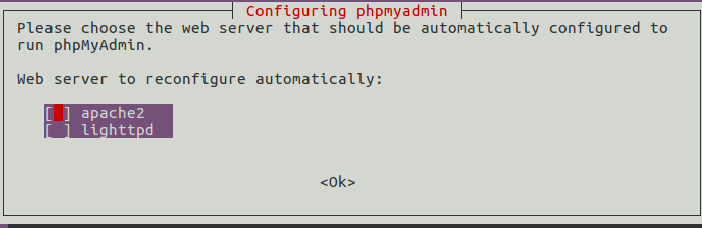
\includegraphics[scale=0.5]{chooseApachePhpMyAdmin}
	}	\caption{Formulario de selección de tipo de servidor web}
\end{figure}
